\setbeamercolor{background canvas}{bg=fitblue}
\begin{frame}
\frametitle{Geometry Shader}
\begin{center}
\Huge {\color{white}Geometry Shader}
\end{center}
\end{frame}
\setbeamercolor{background canvas}{bg=white}

\begin{frame}[fragile]
\frametitle{Geometry shader}
  \scriptsize
	\begin{itemize}
    \item Geometry shader is located between rasterisation and vertex shader (after tessellation).
	  \item It processes primitives - It can access all atributes of all primitive vertices.
    \item It can generate or modify geometry (a point to polygon).
    \item It can be used for various effect (shadows, particle systems, debug draws).
	  \item Geometry Instancing.
	  \item Transform feedback.
	\end{itemize}
	\begin{itemize}
	  \item Geometry shader se nachází za vertex shaderem (za teselací).
	  \item Pracuje po primitivech - má přítup ke všem atributům všech vrcholů vstupního primitiva
	  \item Umožňuje generování geometrie a její úpravu.
	  \item Transformaci bodu na polygon. 
	  \item Používá se pro různé efekty (např. stíny (pomocí stínových těles)).
	  \item Další využití může být v částicových systémech.
	  \item Geometry Instancing.
	  \item Transform feedback.
	\end{itemize}
\end{frame}

\begin{frame}[fragile]
\frametitle{Geometry shader - inputs/outputs}
  \scriptsize
	\begin{itemize}
  \item Type of input primitive has to be specified inside geometry shader.
	\item V Geometry shaderu je nutné specifikovat typ vstupního primitiva.
	{\scriptsize
\begin{minted}[bgcolor=bg]{packages/graphics.py:GLShaderLexer -x}
layout(points,invocations=N)in;//vstupni primitivum bude bod
//points, lines, lines_adjacency, triangles, triangles_adjacency
//invocations - kolikrat bude GS spusten na jedno primitivum
	\end{minted}
	}
	\item Type of output primitive has to be also specified as well as maximal number of vertices.
	\item Také je nutné definovat výstupní primitivum a maximální počet výstupních vertexů.
	{\scriptsize
\begin{minted}[bgcolor=bg]{packages/graphics.py:GLShaderLexer -x}
layout(triangle_strip,max_vertices=4)out;//vystup je sekvence troj.
//points, line_strip, triangle_strip
	\end{minted}
	}
	\end{itemize}
\end{frame}

\begin{frame}[fragile]
\frametitle{Geometry shader - a point to square}
	\begin{figure}[h]
		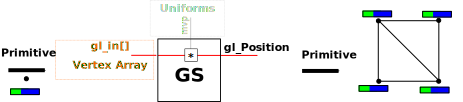
\includegraphics[width=9cm,keepaspectratio]{pics/geometryShader/gs.pdf}
	\end{figure}
  \scriptsize

	{\scriptsize
\begin{minted}[bgcolor=bg]{packages/graphics.py:GLShaderLexer -x}
#version 430

layout(points)in;
layout(triangle_strip,max_vertices=4)out;

void main(){
  gl_Position=mvp*(gl_in[0].gl_Position+vec4(-1,-1,0,0));
  EmitVertex();
  gl_Position=mvp*(gl_in[0].gl_Position+vec4(-1,+1,0,0));
  EmitVertex();
  gl_Position=mvp*(gl_in[0].gl_Position+vec4(+1,-1,0,0));
  EmitVertex();
  gl_Position=mvp*(gl_in[0].gl_Position+vec4(+1,+1,0,0));
  EmitVertex();
  EndPrimitive();
}
	\end{minted}
	}
\end{frame}

\begin{frame}[fragile]
\frametitle{Geometry shader - fullscreen quad}
	{\scriptsize
\begin{minted}[bgcolor=bg]{packages/graphics.py:GLShaderLexer -x}
#version 430
layout(points)in;
layout(triangle_strip,max_vertices=4)out;
void main(){
  gl_Position=vec4(-1,-1,0,1);EmitVertex();
  gl_Position=vec4(-1,+1,0,1);EmitVertex();
  gl_Position=vec4(+1,-1,0,1);EmitVertex();
  gl_Position=vec4(+1,+1,0,1);EmitVertex();
  EndPrimitive();
}
	\end{minted}
	}
	{\scriptsize
\begin{minted}[bgcolor=bg]{packages/c_cpp.py:CppLexer -x}
glCreateVertexArrays(1,&emptyVAO);
//...
glBindVertexArray(emptyVAO);//empty VAO
glDrawArrays(GL_POINTS,0,1);
glBindVertexArray(0);
	\end{minted}
	}
\end{frame}

\begin{frame}[fragile]
\frametitle{shadow volumes - zfail}
  \begin{figure}[h]
    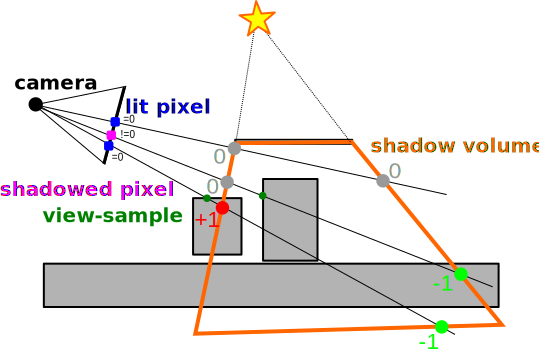
\includegraphics[width=11cm,keepaspectratio]{pics/geometryShader/shadowvolume.pdf}
  \end{figure}
\end{frame}

\begin{frame}[fragile]
\frametitle{Geometry shader - shadow volumes}
  \begin{columns}[T]
    \begin{column}{.44\textwidth}
	    {\tiny
\begin{minted}[bgcolor=bg]{packages/graphics.py:GLShaderLexer -x}
#version 330
layout(triangles)in;
layout(triangle_strip,max_vertices=10)out;
uniform mat4 MVP,M;//matice
uniform vec4 LightPosition;//pozice svetla
void main(){
  vec4 LP=M*LightPosition;
  vec4 p[6];
  p[0]=gl_in[0].gl_Position;//triangle points
  p[1]=gl_in[1].gl_Position;
  p[2]=gl_in[2].gl_Position;
  p[3]=vec4(gl_in[0].gl_Position.xyz*LP.w-LP.xyz,0);//in infinity
  p[4]=vec4(gl_in[1].gl_Position.xyz*LP.w-LP.xyz,0);
  p[5]=vec4(gl_in[2].gl_Position.xyz*LP.w-LP.xyz,0);
  vec3 N=normalize(cross((p[1]-p[0]).xyz,(p[2]-p[0]).xyz));
  float Distance=dot(N,LP.xyz)-dot(N,p[0].xyz);
  if(Distance<=0){//otocime volume vnitrkem ven
    vec4 c=p[0];p[0]=p[1];p[1]=c;
    c=p[3];p[3]=p[4];p[4]=c;
  }
  gl_Position=MVP*p[0];EmitVertex();
  gl_Position=MVP*p[1];EmitVertex();
  gl_Position=MVP*p[3];EmitVertex();
  gl_Position=MVP*p[4];EmitVertex();
  gl_Position=MVP*p[5];EmitVertex();
  gl_Position=MVP*p[1];EmitVertex();
  gl_Position=MVP*p[2];EmitVertex();
  gl_Position=MVP*p[0];EmitVertex();
  gl_Position=MVP*p[5];EmitVertex();
  gl_Position=MVP*p[3];EmitVertex();
  EndPrimitive();
}
    	\end{minted}
   	}
    \end{column}
    \begin{column}{.48\textwidth}
	    \begin{figure}[h]
    		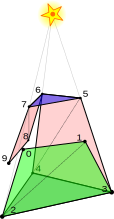
\includegraphics[width=3cm,keepaspectratio]{pics/geometryShader/PerTriangle.pdf}
    	\end{figure}
    \end{column}
  \end{columns}

\end{frame}

